\documentclass[a4paper, 12pt]{report}
\usepackage[utf8]{inputenc}
\usepackage[T1]{fontenc}

\usepackage{xcolor}
\usepackage{afterpage}

\usepackage{relsize}
\usepackage{moresize}

\usepackage{graphicx}
\usepackage{geometry}

% [CHANGE] The title of your thesis. If your thesis has a subtitle, then this
% should appear right below the main title, in a smaller font.
\newcommand{\theTitle}{The first sentence \\
\vspace{0.5em}
the second sentence}
\newcommand{\theSubTitle}{a smaller subtitle}


% [CHANGE] Your full name. In case of multiple names, you can include their
% initials as well, e.g. "Robin G.J. van Achteren".
\newcommand{\theAuthor}{Robin van Achteren}

% [CHANGE] Your student ID, as this has been assigned to you by the UvA
% administration.
\newcommand{\theStudentID}{9123456}

% [CHANGE] The name of your supervisor(s). Include the titles of your supervisor(s),
% as well as the initials for *all* of his/her first names.
\newcommand{\theSupervisor}{Prof. dr. ir. R.J.H. Scha} % Dr. Ing. L. Dorst

% [CHANGE] The address of the institute at which your supervisor is working.
% Be sure to include (1) institute (is appropriate), (2) faculty (if
% appropriate), (3) organisation name, (4) organisation address (2 lines).
\newcommand{\theInstitute}{
Institute for Logic, Language and Computation\\ %Informatics Institute
Faculty of Science\\
University of Amsterdam\\
Science Park 907 \\ % Science Park 904\\
1098 XG Amsterdam % 1098 XH  Amsterdam
}

% [CHANGE] The date at which you will finalize and submit your thesis.
\newcommand{\theDate}{Jan, 2021}

\begin{document}
\pagestyle{empty}
% Page I

% This page should contain your title and name and will create a thumbnail
% which should be readable at https://scripties.uba.uva.nl/



    \newgeometry{margin=1cm}
    \thispagestyle{empty}
    
    % [CHANGE]
    % You can also use one of the other background colors, 
    % preferably one that fits with your cover-image
    % see https://en.wikibooks.org/wiki/LaTeX/Colors for suggestions
    \pagecolor{black}\afterpage{\nopagecolor}
 
    \begin{minipage}[t][0.8\paperheight]{0.8\paperwidth}
        \begin{center}
        
                  %% Print the title a at the top in white.
                  {\color{white} \fontsize{52}{104}\selectfont \textbf{\theTitle} }
               
                  \vspace{0.2\paperheight}
                  
                  % [CHANGE]
                  % Replace this image with one that is relevant for your research, 
                  % If possible, use one of your own illustrations
                 
                  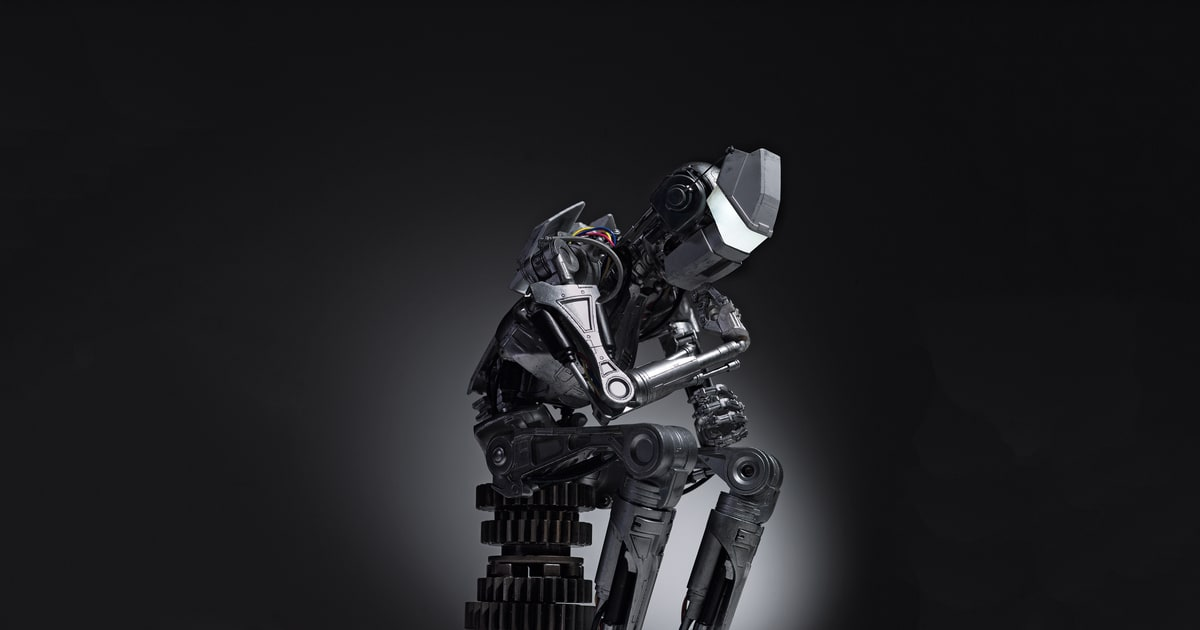
\includegraphics[width=0.75\paperwidth]{augmented-intelligence}
                  
                   %% Print the author at the bottom 
                  \vspace{0.2\paperheight}
                  
                 {\color{white} \fontsize{24}{48}\selectfont \textbf{\theAuthor} }
        \end{center}
    \end{minipage}   
   
    \restoregeometry
    
\newpage

% Page II

\newgeometry{margin=1cm}
\vspace*{0.8\textheight}
\noindent
Layout: typeset by the author using \LaTeX. \\
Cover illustration: Unknown artist 
\restoregeometry

\newpage

% Page III
\begin{center}

\vspace{2.5cm}


\begin{Huge}
% see definition at beginning of document
\theTitle
\end{Huge} \\

\vspace{0.5 cm}

\begin{Large}
\theSubTitle
\end{Large}

\vspace{1.5cm}

% see definition at beginning of document
\theAuthor\\
% see definition at beginning of document
\theStudentID

\vspace{1.5cm}

% [DO NOT CHANGE]
Bachelor thesis\\
Credits: 18 EC

\vspace{0.5cm}

% [DO NOT CHANGE] The name of the educational programme.
Bachelor \textit{Kunstmatige Intelligentie} \\
\vspace{0.25cm}

\includegraphics[width=0.075\paperwidth]{uva_logo} \\
\vspace{0.1cm}

% [DO NOT CHANGE] The address of the educational programme.
University of Amsterdam\\
Faculty of Science\\
Science Park 904\\
1098 XH Amsterdam

\vspace{2cm}

\emph{Supervisor}\\

% see definition at beginning of document
\theSupervisor

\vspace{0.25cm}

% see definition at beginning of document
\theInstitute

\vspace{1.0cm}

% see definition at beginning of document
\theDate

\end{center}
\newpage

\pagenumbering{arabic}
\setcounter{page}{1}

\chapter{Introduction}
\chapter{Conclusion}

\end{document}
